% !TeX spellcheck = de_CH_frami

\section{CMOS Technologie (Kap. 3)}

\begin{minipage}[t]{0.5\textwidth}
	\textbf{Oberflächenbeschichtgung}\\
	Epitaxie, Oxidation oder Abscheideverfahren\\ [2ex]
	\textbf{Fotolithografie}\\
	Auftragen von Fotolack, anschliessend belichten\\ [2ex]
	\textbf{Ätzen}\\
	Abtragen der Beschichtung
	\begin{figure}[H]
		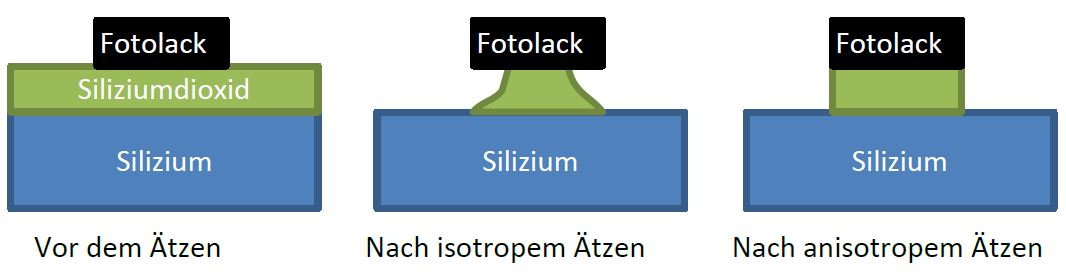
\includegraphics[width=0.8\linewidth]{chapters/Technologie/images/Aetzen}
	\end{figure}
	\begin{tabular}{|l|l|}
		\hline
		\textbf{Bezeichnung}&\textbf{Ätzverfahren}\\ \hline
		Isotropes Ätzen&nasschemisches Ätzen\\ \hline
		Anisotropes Ätzen&Plasmaätzen\\ \hline
	\end{tabular}\\ [2ex]
	\textbf{Dotieren}\\
	Anschluss der Schicht erstellen\\ [2ex]
	\textbf{Säubern der Wafer}\\
\end{minipage}
\begin{minipage}[t]{0.5\textwidth}
	\textbf{Ablauf CMOS Herstellungsprozess}\\
	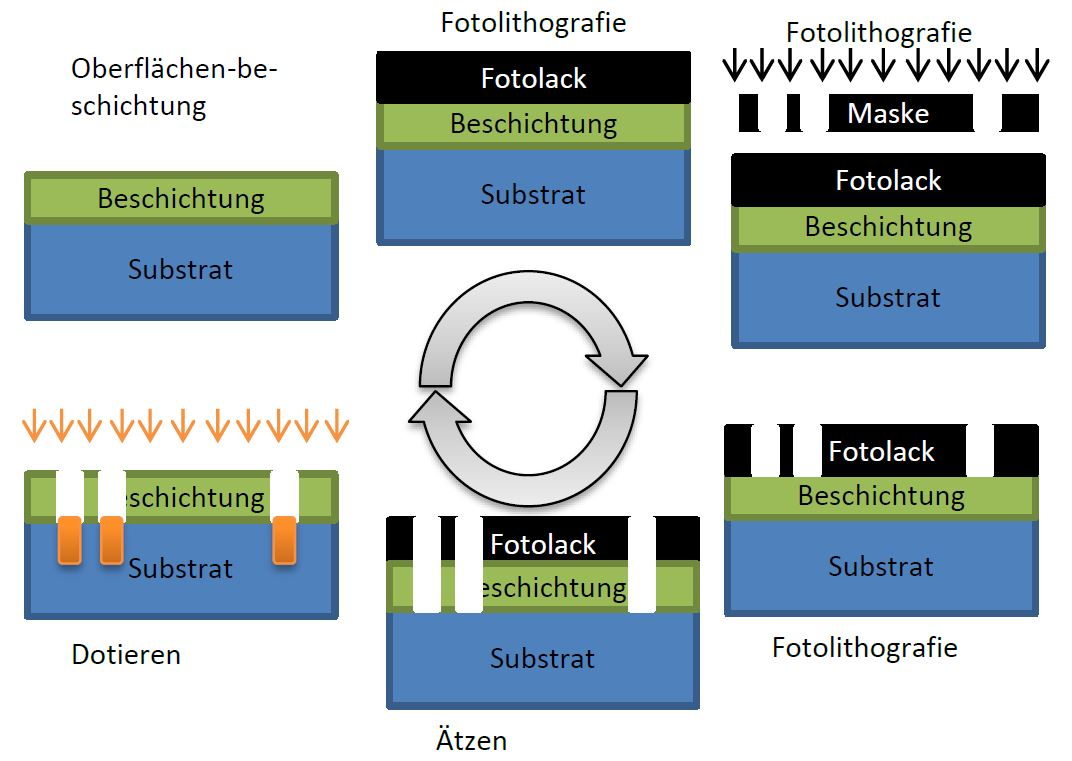
\includegraphics[width=1\textwidth, right]{chapters/Technologie/images/Verarbeitung}
	\textbf{CMOS Technologie - Dotierung}\\
	\begin{tabular}{|l|l|l|}
		\hline
		\textbf{Wertigkeit}&\textbf{Dotierung}&\textbf{Material}\\ \hline
		3&p&Bor (B)\\ \hline
		4&-&Silizium (Si)\\ \hline
		5&n&Arsen (As)\\ \hline
	\end{tabular}
\end{minipage}

\section{Passive Schaltungselemente in CMOS (Kap. 4)}

\begin{minipage}[c]{0.22\textwidth}
	Absolute Genauigkeit:\\Relative Genauigkeit:
\end{minipage}
\begin{minipage}[c]{0.06\textwidth}
	$\pm \SI{20}{\percent}$\\ $\pm \SI{1}{\percent}$
\end{minipage}
\begin{minipage}[c]{0.5\textwidth}
	(Wert vom einzelnen Element)\\(Verhältnis von Elementen zueinander)
\end{minipage}\\[1ex]
Da Verhältnisse sehr genau sind, werden sie in der Schaltungstechnik intensiv genutzt.

\subsection{Kapazitäten}
Auf einem Chip bilden sich zwischen zwei voneinander isolierten Elektroden Kapazitäten.
\\[2ex]
\begin{minipage}[c]{0.55\textwidth}
	\begin{tabular}{|l|l|}
		\hline
		Poly-Poly-Kapazität ($Si$-$SiO_2$-$Si$) & $C'' \approx \SI{1}{\femto \farad \per \micro \meter ^2}$\\ \hline
		MOS-Kapazität (Gate-Gateoxid-Kanal) & $C'' \approx \SI{10}{\femto \farad \per \micro \meter ^2}$\\ \hline
		MIM-Kapazität (Metall-Isolator-Metall) & $C'' \approx \SI{1}{\femto \farad \per \micro \meter ^2}$ \\ \hline
	\end{tabular}
\end{minipage}
%\begin{minipage}[c]{0.35\textwidth}
%	Poly-Poly-Kapazität ($Si$-$SiO_2$-$Si$)\\
%	MOS-Kapazität (Gate-Gateoxid-Kanal)\\
%	MIM-Kapazität (Metall-Isolator-Metall)
%\end{minipage}
%\begin{minipage}[c]{0.2\textwidth}
%	$C'' \approx \SI{1}{\femto \farad \per \micro \meter ^2}$\\
%	$C'' \approx \SI{10}{\femto \farad \per \micro \meter ^2}$\\
%	$C'' \approx \SI{1}{\femto \farad \per \micro \meter ^2}$
%\end{minipage}
\begin{minipage}[c]{0.45\textwidth}
	\uline{\textbf{Legende:}}\\
	$C''$: spezifische Kapazität pro Flächeneinheit\\
	$d$:   Plattenabstand (meist durch Herstellung gegeben)
	%
\end{minipage}
\\[2ex]
\begin{minipage}[c]{0.55\textwidth}
	\uline{\textbf{Formeln:}}\\
	Kapazität/Fläche: $C'' = \frac{\epsilon}{d} = \frac{\epsilon_0 \cdot \epsilon_r}{d}$\\
	Kapazität: \hspace{11.5mm}$C = C'' \cdot A$
\end{minipage}
\begin{minipage}[c]{0.45\textwidth}
	\uline{\textbf{Konstanten:}}\\
	$\epsilon_0 = 8.85 \cdot 10^{-12} \SI{}{\farad / \meter}$\\
	$\epsilon_r = \SI{3.9}{}$ (für Siliziumoxid)
\end{minipage}
\\[2ex]
Neben der gewünschten Kapazität hat jeder Plattenkondensator auch unerwünschte Streukapazitäten. 
Beim Chip fällt vor allem die Streukapazität zwischen der unteren Elektrode und dem Substrat ins Gewicht.

\subsection{Widerstände}
Unerwünscht auf dem Chip, da hoher Platzbedarf und Wärmeentwicklung.
\\[2ex]
\begin{minipage}[c]{0.55\textwidth}
	\begin{tabular}{|l|l|}
		\hline
		Poly-Widerstand & $R_\square \approx \SI{10}{\Omega \per}\square$\\ \hline
		HR-Poly-Widerstand & $R_\square \approx \SI{1}{\kilo\Omega \per}\square$\\ \hline
		P-Diffusions-Widerstand & $R_\square \approx \SI{100}{\Omega \per}\square$\\ \hline
		N-Diffusions-Widerstand & $R_\square \approx \SI{100}{\Omega \per}\square$\\ \hline
		N-Well-Widerstand & $R_\square \approx \SI{1}{\kilo\Omega \per}\square$\\ \hline
	\end{tabular}
\end{minipage}
%\begin{minipage}[c]{0.22\textwidth}
%	Poly-Widerstand\\HR-Poly-Widerstand\\P-Diffusions-Widerstand\\N-Diffusions-Widerstand\\N-Well-Widerstand
%\end{minipage}
%\begin{minipage}[c]{0.33\textwidth}
%	$R_\square \approx \SI{10}{\Omega \per}\square$\\
%	$R_\square \approx \SI{1}{\kilo\Omega \per}\square$\\
%	$R_\square \approx \SI{100}{\Omega \per}\square$\\
%	$R_\square \approx \SI{100}{\Omega \per}\square$\\
%	$R_\square \approx \SI{1}{\kilo\Omega \per}\square$
%\end{minipage}
\begin{minipage}[c]{0.45\textwidth}
	\uline{\textbf{Legende:}}\\
	$R_\square:$ spezifischer Widerstand einer quadratischen Fläche\\\\
	\uline{\textbf{Formel:}}\\
	$R = R_\square \cdot \frac{L}{W}$
\end{minipage}
\\[2ex]
Jeder Widerstand auf dem Chip erzeugt zwangsläufig Streukapazitäten, die es im Design zu berücksichtigen gilt.

\subsection{Induktivitäten}
Mit Standard CMOS-Technologie lassen sich Induktivitäten nicht gut herstellen.
Für RF-Anwendungen werden Spulen eingesetzt, die aber in der Ebene gewickelt werden.
Spulen lassen sich ausserhalb des Chips mit z.B. Bonddrähten realisieren.